\documentclass[12pt,a4paper]{article}
\usepackage{rmpackages}																% usual packages
\usepackage{rmtemplate}																% graphic charter
\usepackage{rmexocptce}																% for DS with cptce eval

%\cfoot{} 													% if no page number is needed
%\renewcommand\arraystretch{1.5}		% stretch table line height

\newcommand{\ritem}{\refstepcounter{enumi}\item[\writeit{} \theenumi .]}

\begin{document}

\begin{header}
TP -- La comète
\end{header}

\begin{multicols}{2}
\begin{center}
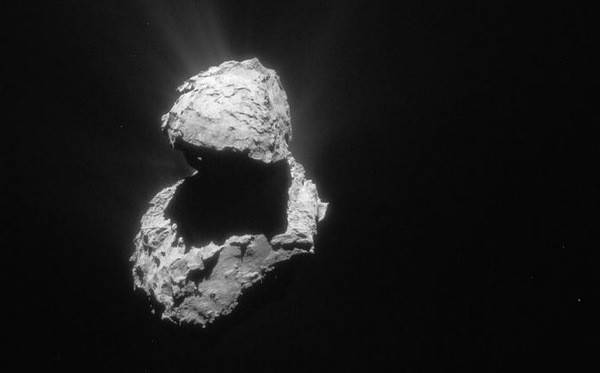
\includegraphics[width=\linewidth]{images/tchouri3.jpg}
\end{center}

En 2014, après dix années de voyage à bord de la sonde européenne Rosetta, le module Philae atteignait enfin sa destination : une comète surnommée \og Tchouri \fg{}.
Première à réaliser l'exploit de se poser à la surface d'une comète, Philae a pu récolter des données qui aident la communauté scientifique à comprendre les processus de formation du système solaire.
La comète Tchouri repassera à proximité de la Terre à la fin de cette année 2021, sans toutefois la menacer.
\end{multicols}

L'objectif de ce TP est d'étudier la trajectoire de quelques objets du système solaire en utilisant Python et les relevés de position effectués par des astrophysiciens.

\begin{enumerate}
\item \rea{}

Copier-coller tout le dossier \og TP Tchouri 1 \fg{} dans votre espace de travail personnel (Ordinateur \textrightarrow{} Ma classe \textrightarrow{} Documents en consultation \textrightarrow{} Physique-Chimie).
\end{enumerate}

\section*{Première trajectoire : la Terre}

\begin{enumerate}[resume]
\ritem \rea{} \app{}

Ouvrir le programme \texttt{position\_planetes.py} avec EduPython et l'exécuter 
\includegraphics[height=0.75\baselineskip]{images/edupython_execute.png}.
Décrire ce qui est représenté sur le graphe.

\ritem \app{}

Les tableaux \texttt{x\_terre} et \texttt{y\_terre} contiennent les abscisses et ordonnées des positions successives de la Terre.
Dans quel autre fichier à votre disposition retrouve-t-on ces coordonnées ?

\emph{Pour lire les fichiers, utiliser Notepad++ : clique droit sur le fichier \textrightarrow{} Edit with Notepad++.}

\ritem \app{}

Quelle durée sépare deux positions successives de la terre ?
% D'après l'entête du fichier trouvé précédemment, quelle durée sépare deux positions successives de la terre ?

\ritem \app{}

Par rapport à quoi sont représentées les positions de la Terre ?
% Quelle est l'origine du repère ?

\ritem \rco{}

Choisir parmi les mots suivants ceux qui permettent de caractériser le mouvement de la Terre autour du Soleil : rectiligne, circulaire, curviligne, uniforme, accéléré, décéléré.
\end{enumerate}

\newpage

\section*{La comète Tchouri}

\begin{enumerate}[resume]

\ritem \app{} \anarai{}

Quel est le rôle de la commande \texttt{plt.plot} ligne 26 ?
Justifier.

\item \anarai{} \rea{}

Les tableaux \texttt{x\_tchouri} et \texttt{y\_tchouri} définis à la ligne 12 contiennent les abscisses et ordonnées des positions successives de la comète Tchouri au cours de son mouvement autour du Soleil.
Modifier le programme ligne 29 pour afficher aussi les positions successives de la comète Tchouri.

\ritem \app{} \anarai{} \val{}

Donner le numéro des lignes du programme permettant de modifier les limites du graphe. 
Modifier le programme pour visualiser l'ensemble des positions de Tchouri.
\end{enumerate}
\begin{appel}
\anarai{}
\end{appel}

\begin{enumerate}[resume]
\ritem \app{} \anarai{}

La vitesse de la comète n'est pas constante au cours de son mouvement autour du Soleil.
À quel endroit est-elle la plus grande ?
Justifier.
\end{enumerate}

\section*{Jupiter}

\begin{enumerate}[resume]
\item \anarai{} \rea{} \val{}

Les tableaux \texttt{x\_jupiter} et \texttt{y\_jupiter} contiennent les abscisses et ordonnées des positions successives de Jupiter au cours de son mouvement autour du Soleil.
Modifier le programme afin de représenter et visualiser l'ensemble des positions successives de Jupiter.

\end{enumerate}

\begin{appel}
\rea{}
\end{appel}

\end{document}

\ritem \app{}

Ouvrir le fichier \texttt{earth.txt} avec Notepad++.
À quoi correspondent les valeurs contenues dans chacune des deux colonnes à partir de la ligne 8 ?
Quelle est l'unité de ces valeurs ?
% Lisez les informations de l'entête du fichier.
% Une unité astronomique permet d'exprimer une durée, une vitesse, une distance ?

\ritem \app{}

Donner l'intervalle de temps qui sépare les valeurs de deux lignes consécutives.
% Lisez l'entête !
% On aurait pu rajouter une colonne devant les positions XY qui indique le temps écoulé depuis la première position. Quelles valeurs aurait-on mis dans cette colonne ?

\ritem \app{} \anarai{} \rea{}

%Exprimer en années la durée sur laquelle s'étalent les données de l'ensemble du fichier.
À un mois près, à quelle date correspond la dernière ligne du document ?
% Combien de jours séparent la première ligne de la deuxième ? De la troisième ? ... De la dernière ?
% Combien y a-t-il de lignes dans le fichier ?